\label{section:azure:databricks}

\textit{Azure Databricks} is an Apache Spark-based analytics platform optimized for the Microsoft Azure cloud services platform \cite{bib:azure:databricks:description}.

Databricks allows full management of Spark clusters, along with online editing of scripts, which are used to create and submit jobs to the cluster.

\subsubsection{Folder structure}
    Databricks provides a single workspace shared across all users.
    It is possible to create and manage folders and files under this workspace.
    
    By default, there are two folders with special permissions already set-up.
    
    \paragraph{Shared}
        All objects stored under the \texttt{Shared} folder are public, meaning that all users have read, write and execute permissions on them.
        
        This folder can be used as a quick way to share items between users, especially if they have different or incompatible permissions.
        
    \paragraph{Users}
        The \texttt{Users} folder contains a subfolder for each user who has access to Databricks.
        
        By default, each user is the administrator of their own folder, but they can also give permissions to other users.

\subsubsection{Coding}
    Databricks allows programming in the following languages:
        \begin{itemize}
            \item Python
            \item Scala
            \item R
            \item SQL
            \item Bash
        \end{itemize}
    
    Scripts are divided into several cells, similarly to a Python notebook.
    
    Each cell must be written in a single programming language, but a script can contain cells in different languages.
    
    In order to specify how a script should be interpreted it is sufficient to write the language used in the first line of the cell.
    
    Figures \ref{fig:azure:databricks:scala}, \ref{fig:azure:databricks:python} and \ref{fig:azure:databricks:bash} show a cell in Scala, one in Python, and one in Bash, respectively.
    These different cells can even belong to the same script.

    \begin{figure}
        \centering
        \begin{subfigure}{0.4\textwidth}
            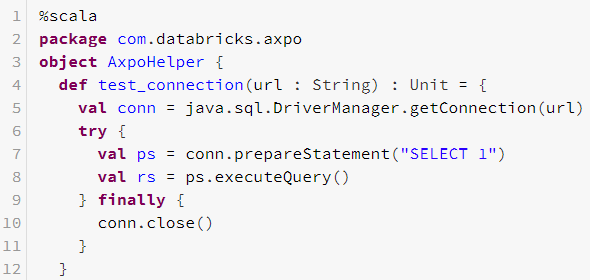
\includegraphics[width=\textwidth]{res/azure/databricks/scala.png}
            \subcaption{Scala}
            \label{fig:azure:databricks:scala}
        \end{subfigure}
        
        \begin{subfigure}{0.4\textwidth}
            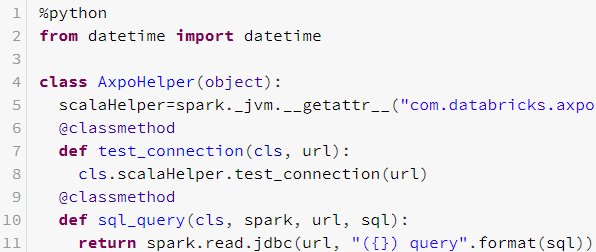
\includegraphics[width=\textwidth]{res/azure/databricks/python.png}
            \subcaption{Python}
            \label{fig:azure:databricks:python}
        \end{subfigure}
        
        \begin{subfigure}{0.4\textwidth}
            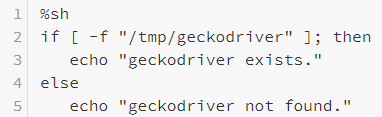
\includegraphics[width=\textwidth]{res/azure/databricks/bash.png}
            \subcaption{Bash}
            \label{fig:azure:databricks:bash}
        \end{subfigure}
        
        \caption{Different scripting languages in Databricks.}
    \end{figure}
    
\subsubsection{Permissions}
    Admins can specify advanced permissions for each folder or even file.
    
    It is possible to assign permissions to both single users and groups.
    
    Figure \ref{fig:azure:databricks:permissions} shows an example of permissions, which are set on a folder called ETL.
    All users belonging the the group ``admins'' can manage the folder and its content, while the user ``Mario P***'' can only read its content.
    
    \begin{figure}
        \centering
        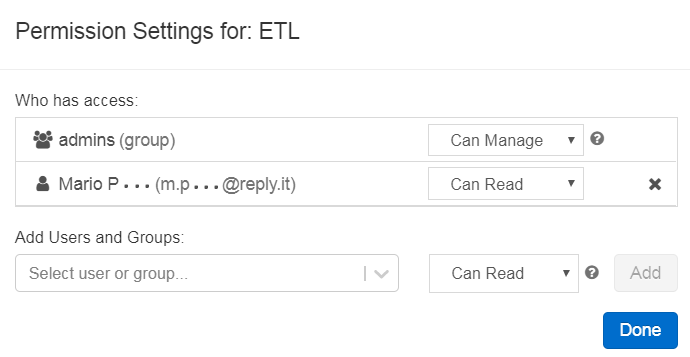
\includegraphics[width=.7\textwidth]{res/azure/databricks/permissions.png}
        \caption{Azure Databricks folder permissions.}
        \label{fig:azure:databricks:permissions}
    \end{figure}
    
    \paragraph{Options}
        There are different permission options.
        These are:
        \begin{enumerate}
            \item No permissions
                \begin{itemize}
                    \item Users cannot do anything with this object
                \end{itemize}
            \item Can Read
                \begin{itemize}
                    \item Users can read and comment notebooks in the folder
                \end{itemize}
            \item Can Run
                \begin{itemize}
                    \item Users can read, comment, attach/detach and run commands in notebooks in the folder
                \end{itemize}
            \item Can Edit
                \begin{itemize}
                    \item In addition to the above, users can also modify notebooks in the folder
                \end{itemize}
            \item Can Manage
                \begin{itemize}
                    \item Users can do all of the above, as well as assign permissions to others
                \end{itemize}
        \end{enumerate}
        
    \paragraph{Groups}
        Permissions can also be assigned at group-level.
        Groups are a collection of users which share the same permissions.
        
        A default group, called ``admins'' has manage permissions on all objects in Databricks.
        Other groups can be freely created and managed.
        
    \paragraph{Default permissions}
        By default, admins have \textit{manage} permissions on all items in Databricks.
        They have full access to any file, which means that they can also see proprietary algorithms or other company secrets.
        
        Each user has also \textit{manage} permissions on their personal folder, under the directory ``Users''.
        This place acts as their personal workspace, in which they can perform any action.
        
        There is also a shared folder in which all users have by default all permissions.
        This folder is useful as a quick way of sharing code between users, especially if they have different permissions, or if they want to share only specific files.

\subsubsection{Execution}
    All scripts create a job identified by an UUID\footnote{Universally Unique Identifier}.
    These jobs are executed on an Apache Spark cluster.
    
    All standard operations of a cluster are available, such as viewing running, queued and completed jobs, inspecting job stages and inspecting and changing cluster configuration.
    
    All of these options can be selected through a standard SparkUI interface, such as the one shown in Figure \ref{fig:azure:databricks:sparkui}.
    
    \begin{figure}
        \centering
        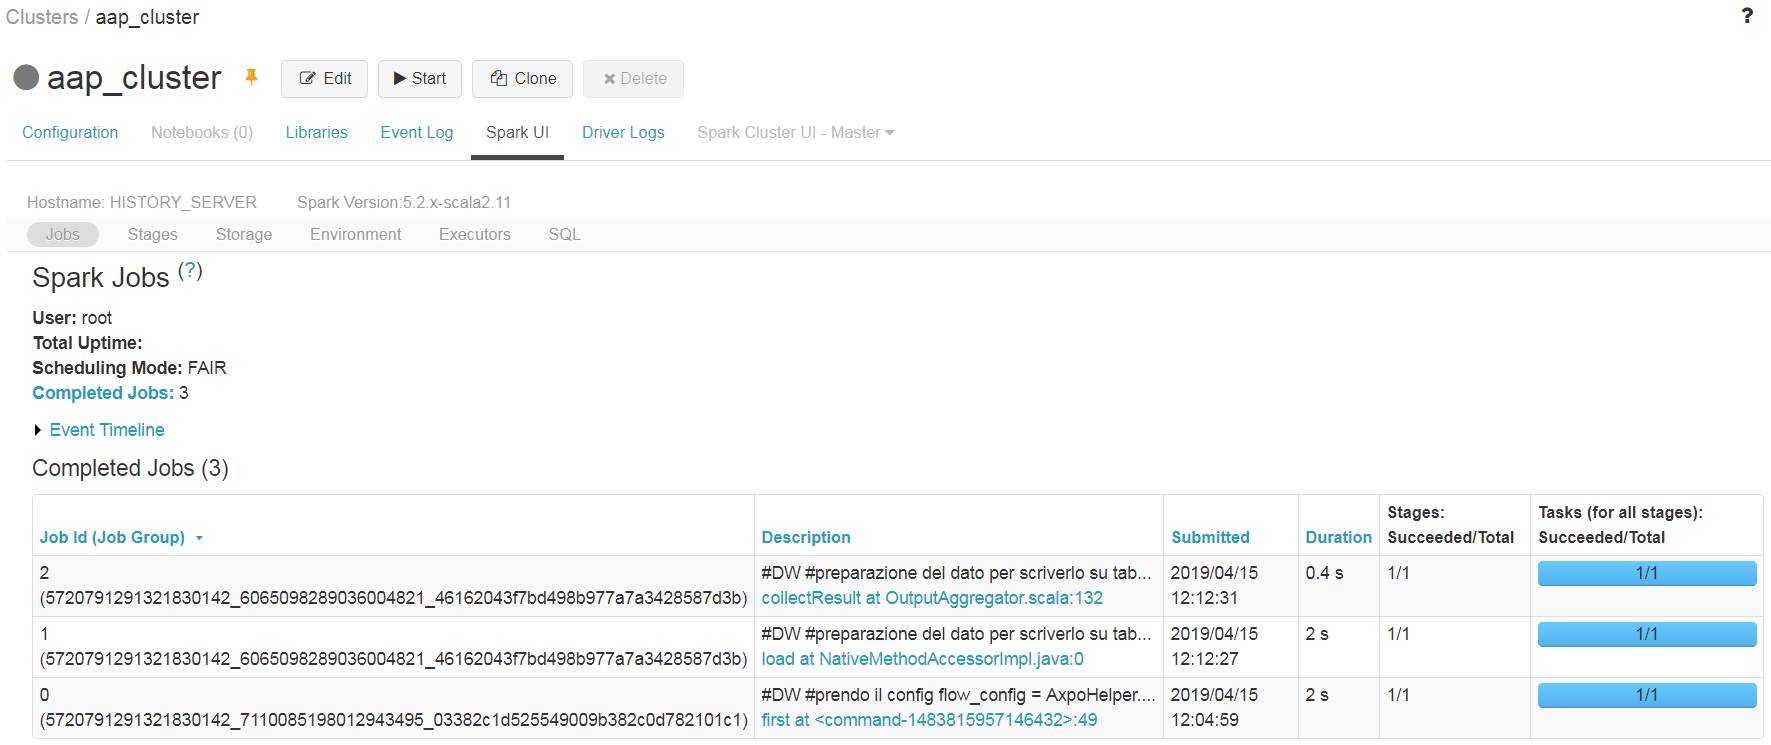
\includegraphics[width=\textwidth]{res/azure/databricks/sparkui.png}
        \caption{Databricks SparkUI interface.}
        \label{fig:azure:databricks:sparkui}
    \end{figure}
    
    \paragraph{Cluster specifications}
        The cluster is composed of two nodes: one is both master and worker, the other serves only as worker.
        Each node has 14 GB RAM available and 4 cores.
        
        One of the most important aspects of Databricks is called \textit{autoscaling}.
        If the cluster is currently executing a computationally demanding task, Databricks may choose to add some workers to increase performance.
        It is possible to set both the minimum and the maximum amount of workers.

        Autoscaling is useful when facing variable loads, since it allows to save up some costs by shutting off some workers that are not needed, whereas in a statically-sized cluster all workers would be constantly active.
        
\subsubsection{Importing/Exporting scripts}
    Databricks allows exporting and importing scripts by directly interacting with the user interface, from which it is possible to export a whole folder in \texttt{zip} format.
    Similarly, it is also possible to import a zipped folder into a different environment.
    Alternatively, a single file can also be directly exported in their native format.
